Maskinens degform ska stänga en Raviolideg med hjälp av två likströmsmotorer. Motorers rotationsenergi ska överföras till degformen med användning av en kugghjulsväxel. Kugghjulsväxel ska bestå av ett kugghjul som sitter på en likströmsmotor och ett kugghjul som ska monteras på baksidan av masinens degform.

Utväxling av kugghjulsväxel räknas med formel:
\begin{center}
\LARGE \textbf{	$ i = \frac{N1}{N2}$}
\end{center}
där i är utväxlingen, N1 är det drivande kugghjulets varvtal och N2 är det drivna kugghjulets varvtal. 

Det är också tänkt att implementera möjligheten att hissa upp och ner maskinens degform. Detta görs för att minska avstånd mellan maskinens degform och pump. För att genomföra detta ska en kuggväxel bestående av två kugghjul och två kuggsträngar användas, se figur.~\ref{maskinens_baksida_metod}

\begin{figure}[ht]
	\begin{center}
		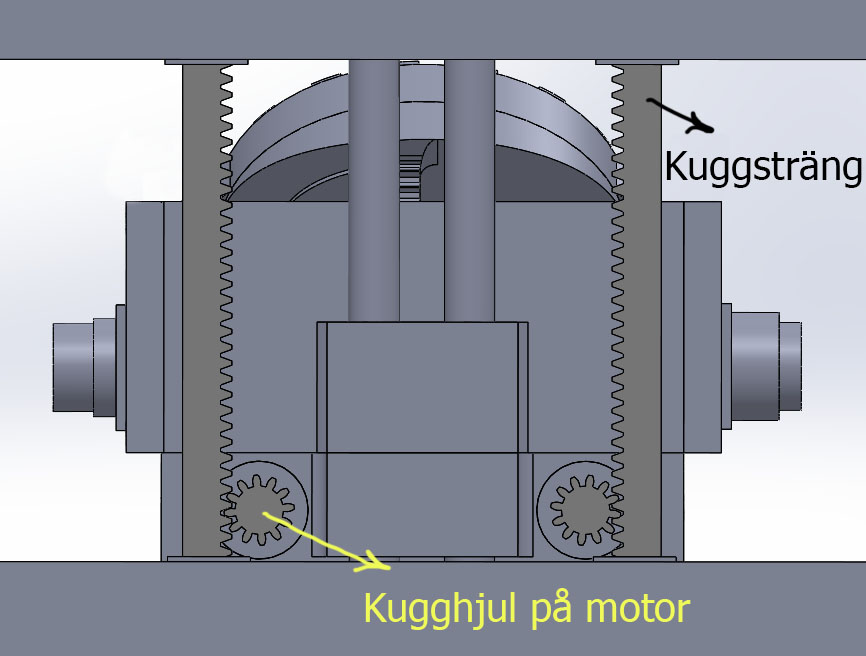
\includegraphics[scale=0.8]{images/maskinBaksida.jpg}
		\caption{Maskinens baksida som innehåller kuggsträngar och kugghjul(kuggväxel)}
		\label{maskinens_baksida_metod}	
	\end{center}
\end{figure}
